% $Id: ESMF_infradataoverview.tex,v 1.7 2004/02/19 00:12:43 svasquez Exp $

\section{Overview of Infrastructure Data Classes}

{\tt Field}, {\tt Bundle}, and {\tt Array} objects 
provide data access and data handling methods.
Their methods are called both from user written
code and from other objects internal to the framework.

A {\tt Field} 
object encapsulates computational and/or observational data together 
with the underlying grid on which it is located.  
A {\tt Field} object provides the
application with both an overall logical view of the entire
dataset, as well as access to processor-local data after decomposition.
It provides methods for configuration, initialization, setting and
retrieving data values, data I/O, intercomponent data 
exchange, data regridding, and manipulation of attributes.

Groups of fields on the same underlying physical grid 
can be collected into a single object called a {\tt Bundle}.  
A {\tt Bundle} provides two major functions: it allows groups of 
{\tt Fields}
to be manipulated using a single identifier, for example during
export or import of data between components; and it allows
data from multiple fields to be packed together in memory 
for higher locality of reference and ease in subsetting operations.
A {\tt Bundle} object contains methods
for setting and retrieving constituent fields, import and export
data exchange during intercomponent communication,
regridding, data I/O, and reordering of data in memory.


\subsection{Programming Model}

The following sections give a high level description of how
the overall application and components will operate,
focusing on how Fields and Bundles are created and used.
This is followed by a more detailed description of how
those functions are encapsulated into internal ESMF 
objects, followed by a detailed API (Application Programming
Interface) listing.

\subsection{Using Fields and Bundles}

\subsubsection{Field Initialization}

The following section describes issues related to
creation and initialization of Fields.

\begin{description}

\item{Framework Initialization}
 
At Framework initialization there is an opportunity to 
specify a configuration file which can contain attribute values 
that affect the
operation of Fields and Bundles.  The most likely used
attributes will control I/O specifications, e.g. 
filenames and file formats defaults.  These can be
queried at run time by the Field and Bundle code.

\item{Field Creation}

All versions of the {\tt ESMF\_FieldCreate} 
routines require a Grid object as input, or require a Grid
be added before most operations involving Fields can be performed.
The Grid contains the information needed to know which 
Decomposition Elements ({\tt DE}s) are participating in 
the processing of this Field, and which subsets of the data
are local to this {\tt DE}.

Requests to access local Field data will not require 
communication overhead; the user code is expected to
query the Grid object to discover what part of the
overall dataset is local to this processor and do
computations based on that data.

The details of how the create process happens depends 
on which of the 
variants of the {\tt ESMF\_FieldCreate} call is used.
Some differences will be discussed below.

\item{Associating constructed data with Fields}

There are versions of the {\tt ESMF\_FieldCreate} interface
which allow user code to specify the initial data values.
The can be constructed or read in data from
outside of the ESMF.  Empty Fields can also be created in
which case the data can be added at some later time.

For versions of Create which do not specify data values,
user code can create an {\tt ESMF\_ArraySpec} object, which
contains information about the Type, Kind, and Rank of the
data values in the array.  Then at Field create time, the
appropriate amount of memory is allocated to contain the
data which is local to each {\tt DE}.

\item{Having Fields Allocate Space for Data}

There are versions of the {\tt ESMF\_FieldCreate} interface
which create the Field based on the input Grid.  The ESMF
can allocate the proper amount of 
space but not assign initial values.  The user code
can then detach the uninitialized buffer, set the
initial data values, and reattach the buffer.

\item{Field Read}

Fields can be created by the {\tt ESMF\_FieldRead}
routine, with options to create the Grid at this time
as well as creating the associated Arrays.

\end{description}

Fields can be created and destroyed
at any time during application execution.  However, the creation
and deletion of Fields will require some time to complete.  
It is not recommended
that Fields are created or destroyed
inside performance-critical computational loops.

Fields and Bundles are used in constructing 
the Import and Export states for component coupling, 
which requires that the 
Fields involved in data exchange be identified, as well as
which Transforms must be performed on them to make the
data compatible with the specifications of
receiving components.  

\subsubsection{Bundle Initialization}

It is not required that {\tt Bundles} be created or used.
{\tt Bundles} offer a way to group {\tt Fields} which share a
common {\tt Grid}, and optionally to pack the {\tt Field} data
together in a single buffer.

\begin{description}

\item{Bundle Creation from Existing Fields}

After creating multiple Fields, Bundles can be created
by calling the {\tt ESMF\_BundleCreate} subroutine.  There are
options to create a {\tt Bundle} which simply references
the data buffers of the existing {\tt Fields}, 
or the Bundle can make a separate copy of the data in a private 
Bundle data buffer.  If a data copy is made, there are options to
control the interleaving of the Field data in the Bundle data buffer.

All Fields in a bundle must share the same underlying Grid.
If the Bundle has a private data buffer, then the Fields must
all share a compatible mapping of data onto the Grid as well.

\end{description}

\subsubsection{Use During Execution}

Access to data is similar for {\tt Fields} and {\tt Bundles} with
packed data.  It is described below using the {\tt Field}
routines in the examples, but corresponding {\tt Bundle} level
routines exist.  To access data in a
Bundle which is not packed, the user must loop over the
Fields in the Bundles, querying for each
constituent Field and then using the Field level data interfaces.

\begin{description}

\item{Accessing Field Data}

The user code on each DE calls the {\tt ESMF\_FieldGridQuery}
routine to find out about the local subset of the data, including
the number of items, the extents
of the dimensions, and the corresponding coordinates of this
decomposition.

The user code can then call {\tt ESMF\_FieldDataDetach} to
begin iterating through the data.  This routine returns a
pointer to the buffer and marks the data as "in use by
the user code".  The ESMF cannot read or write that
data until {\tt ESMF\_FieldDataAttach} is called.  Once the data
is reattached the framework can use the data in regridding 
operations, halo updates, etc.  

There is a data access option, {\tt ESMF\_FieldDataDetachCopy}
which returns a copy of the data buffer and does not mark the
Field data as detached or in use in any way.  The ESMF 
allocates space for this data buffer, so it becomes the
responsibility of the calling code to release that space 
when finished with it.

\end{description}

\subsubsection{Finalization}

\begin{description}

\item{Field Deletion}

There is a {\tt ESMF\_FieldDestroy} subroutine which releases
any data buffers which were allocated or copied by this Field,
and deletes the Field object.  Since the Grid can be shared
amongst multiple Fields, the Grid is not deleted by this call.

\item{Bundle Deletion}

If Bundles are used, the user must call the 
{\tt ESMF\_BundleDestroy} subroutine before deleting any constituent
Fields.  If a private Bundle data buffer exists, the space is
freed and all resources associated with the Bundle are released.
The constituent Fields are not deleted by this call, since they
can be contained by multiple Bundles.

\end{description}

\subsection{Attributes}

Attributes are implemented in the Base class so they can be attached to
any object in the system which is built on the Base object.  (This is true
for all deep objects in the system.)  Attributes are created by making a
private copy of the information provided during the Set call.  Lists of
values are supported, but they are not intended for problem-sized
data arrays.   Data is also copied during a Get operation.

There are routines for setting and getting single values and lists of
int/I4, double/R8, and logical (ESMF\_Logical) types, and char */character
strings.  (Arrays of character strings are not supported.)

Attributes can be gotten by name.  The type and count can also be queried
by name and then a specific Get call can be made.  (The arguments to the
Get routines are typed and overloaded, so the type of the Attribute must
match the type of the argument receiving it.)

A count of all Attributes associated with an object can be returned, and
then Attributes can also be queried and retrieved by number, for iterating
an unknown Attribute list.

For this release, Fields, Bundles, and States have Attribute support enabled.

\input{../Infrastructure/Base/doc/ESMF_Base_fapi}


\subsection{Data Class Communication Methods}

The following methods operate on Data Class objects, including
{\tt ESMF\_Bundle}s, {\tt ESMF\_Field}s, and {\tt ESMF\_Array}s.
The {\it Regrid} method computes new data values based on a source
and destination grid, and a Regridding Method.  The {\it Halo} 
method updates ghost-cell or halo regions; data which is computed
by a one DE but a copy is needed by another DE to do computations.
The {\it Redistribution} method moves data from one DE to another
when the decomposition of identical Grids is different or the
index ordering of the data is to be changed.  No data
interpolation is done during this process.

There is a common object handle, an {\tt ESMF\_RouteHandle}, which
allows the communication patterns to be precomputed during initialization
and the information stored in that RouteHandle.
By specifying the correct RouteHandle at execution time, only
the source and destination data pointers must be supplied and the
runtime overhead is minimized.

In the following methods, the Bundle and Field code cascades down
through the Array code, so that the actual computations exist in
only one place in the source.

\subsubsection{Regrid}

% $Id: Regrid_desc.tex,v 1.5 2004/05/17 22:34:53 jwolfe Exp $
%
% Earth System Modeling Framework
% Copyright 2002-2003, University Corporation for Atmospheric Research, 
% Massachusetts Institute of Technology, Geophysical Fluid Dynamics 
% Laboratory, University of Michigan, National Centers for Environmental 
% Prediction, Los Alamos National Laboratory, Argonne National Laboratory, 
% NASA Goddard Space Flight Center.
% Licensed under the GPL.


Bundle, Field, and Array classes all have regrid methods that transform their
data from one {\tt ESMF\_Grid} to another.  Regrid operations compute addresses
and interpolation weights for remapping between different grids.  All
the information necessary to perform a regridding, including {\tt ESMF\_Routes}
to collect non-local data and the addresses and weights, are contained in the
{\tt ESMF\_RouteHandle} which is returned to the user.  Since interpolation
weights are based solely on the grids' geometries and addresses are stored
as offsets, regrids can be shared by data classes providing
they have the same {\tt ESMF\_Rellocs}.  The algorithms and some of the
implementation in ESMF's regridding routines are adapted from a software package
called SCRIP that was developed at the Los Alamos National Laboratory by Phil
Jones.  However, SCRIP is a serial code and the ESMF regridding routines have
been parallelized.



\subsubsection{Halo}

% $Id: ArrayHalo_desc.tex,v 1.3 2004/06/03 22:33:15 cdeluca Exp $

\label{sec:halo}
Halo operations update ghost cell or halo regions at the boundaries
of a local data decomposition.  Halo regions are to be considered
read-only by the local process; their data values can be used to
compute the new values for cells which are local to this process,
but they cannot be updated except by a halo operation.  Haloing is
supported at the Array and Field level.  

\subsection{Halo Domains}

Array objects can have an optional {\bf halo width} which defines
what part of the Array is the {\bf exclusive domain}, the {\bf computational
domain}, and the {\bf total domain}.  With no halo region, all these are
the same and equal to the total size of the Array.  The domains are
defined as follows.

\begin{itemize}

\item {\bf Exclusive}  The exclusive domain is the subset of the
Array which is never read by any other DE.  

\item {\bf Computational}  The computational domain
is the subset of the Array which is read and written by the current DE.

\item {\bf Total}  The total domain includes the region where data is 
updated from another DE during a halo operation and read but not 
updated by the current DE.  

\end{itemize}

Figure \ref{fig:halo} illustrates these concepts.

Halo domain information must be stored at the Array level to
support operations such as the gather, which collects
decomposed parts of a logically contiguous object onto a single DE.
Only the computational domain is copied since the halo regions are
duplicated data.  The exclusive domain is guaranteed to never be
the source of data for a halo operation, so no synchronization
of updates to those data items needs to be done.  The total
domain is the actual memory size allocated for the Array,
and is used when computing offsets for subdomains within the Array.

\begin{center}
\begin{figure}
\caption{Diagram showing how ESMF exclusive, computational,
and total domains are defined.  }
\label{fig:halo}
\scalebox{1.0}{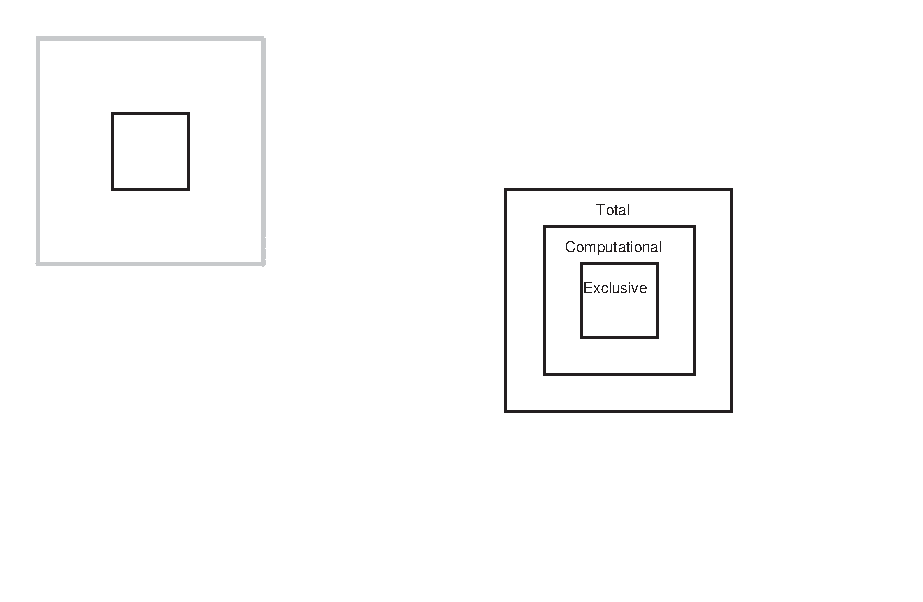
\includegraphics{Field_halo.eps}}
\end{figure}
\end{center}




\subsubsection{Redistribution}

% $Id: ArrayRedist_desc.tex,v 1.7 2005/12/21 23:23:23 jwolfe Exp $


As the name implies, Redistribution operations move data from one distribution,
or decomposition, to another.  The distribution of the data may differ in several 
ways:
 \begin{description}

  \item The data could be decomposed across multiple DEs differently.  In this
        case, the source data might be decomposed by a 3 by 2 DELayout and be
        redistributed onto a 1 by 6 DELayout.

  \item The data could have different index orderings.  For example, the data
        might be reordered from IJK to KIJ, where the source data is
        dimensioned srcData(ni,nj,nk) and is redistributed to dstData(nk,ni,nj).

  \item Different indices of the data could be decomposed.  Source data
        decomposed only in the first index could be redistributed to being
        only in the second or third index.  For example, if both the source
        and destination data are decomposed by a 4 by 1 DELayout but the source
        applies the decomposition to the first index and the destination
        applies it to the second, then the source data will be locally
        dimensioned srcData(ni/4,nj,nk) and redistributed to dstData(ni,nj/4,nk).

 \end{description}

In all of these situations, the source and destination data structures are
required to have identical global sizes but not DE-local sizes.  Although
illustrations of Redistribution may look very similar to Regridding (please
see Figure \ref{fig:Redist}),

\begin{center}
\begin{figure}
\label{fig:Redist}
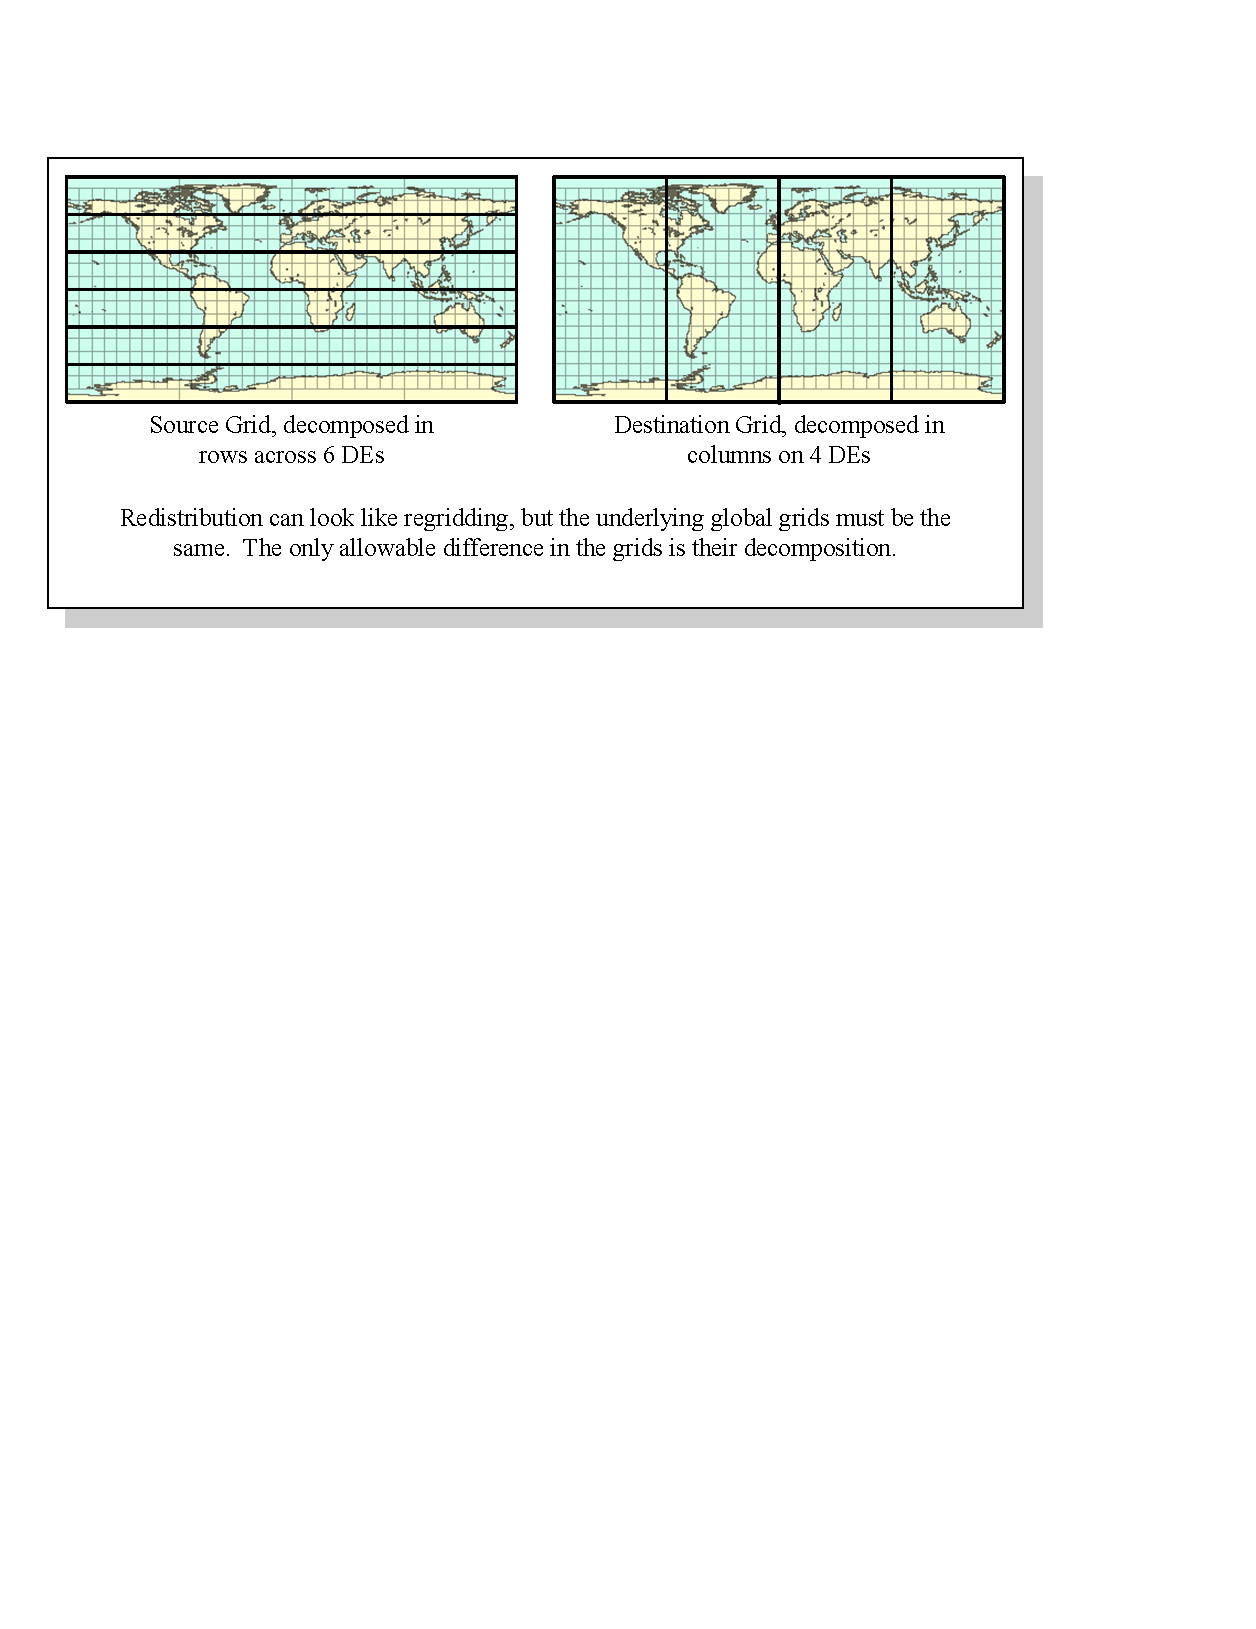
\includegraphics{Redist}
\caption{Illustration of redistribution of data. }
\end{figure}
\end{center}

Redistribution methods involve only data movement; no interpolation, data
binning, or averaging is performed.  For data associated with physical locations
on a Grid, this means the source and destination Grids must have identical
global coordinates.  Like Haloing and other high level communication routines,
Redistribution is supported at the Array, Field, and Bundle levels. 



\subsubsection{Gather, Scatter, etc}

There are lower level communication routines which have methods
at the Array level to simplify the interfaces to the user code.
Field and Bundle methods may be added if required.
The full list of possible communication routines in this category
are Gather, AllGather, Scatter, Reduce,
AllReduce, Broadcast, and AllToAll.

\newpage
\subsection{Object Model}

The following is a simplified UML diagram showing the relationships among
ESMF Field, Grid and Bundle classes.  See Appendix A, {\it A Brief 
Introduction to UML},
for a translation table that lists the symbols in the diagram and their 
meaning.

\begin{center}
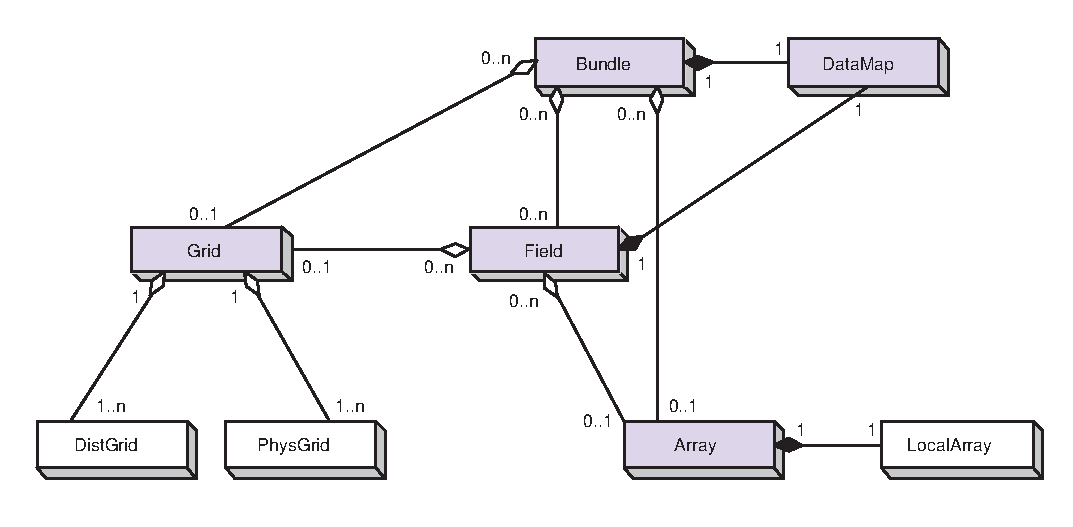
\includegraphics{Bundle_obj.eps}   
\end{center}

